\section{Conclusion}

\subsection{Open Source}

Given the open source nature of ATS, all of the Flying Squid project is open source. Code can be found at \url{https://github.com/FlyingSquid/}.

\subsection{Benchmarking}

The Flying Squid  benchmarking infrastructure involves using ApacheBench to time file downloads through ATS with caching turned on running on an AWS EC2 instance. We hosted test files of specific sizes on our public Github organization repository.

\begin{figure}[H] \centering
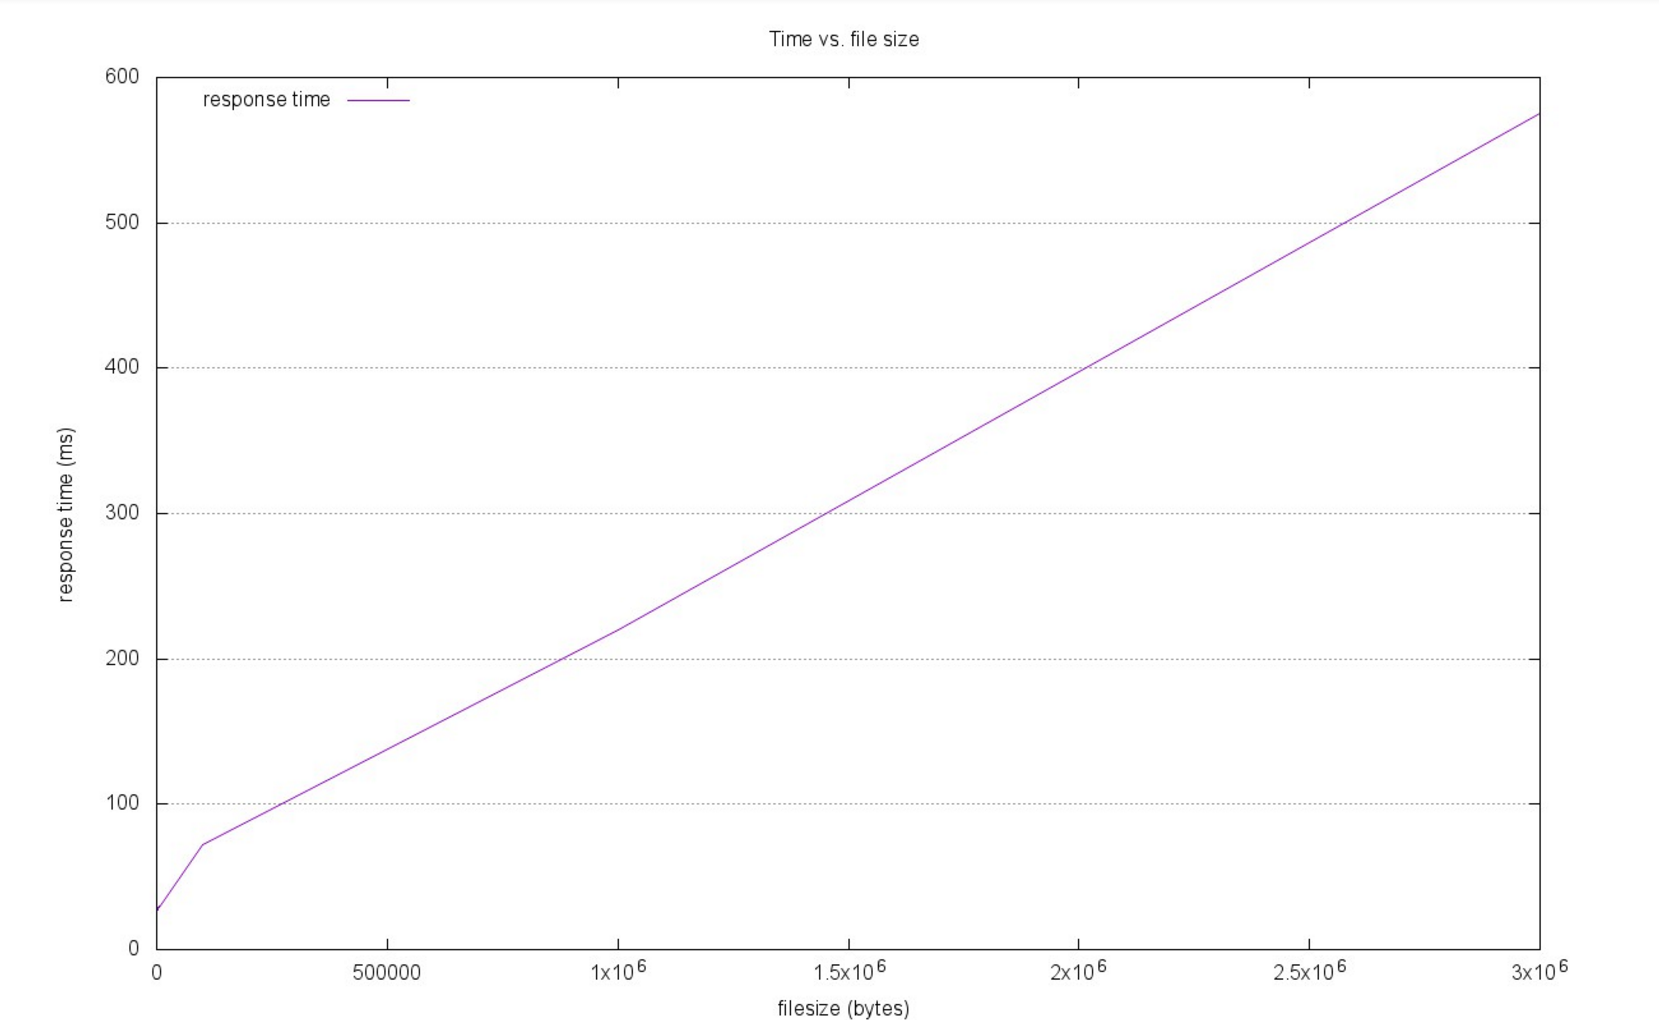
\includegraphics[width=\textwidth]{Benchmarking1}
\caption{Initial Benchmarks: ATS graph of file size vs mean service time}
\end{figure}


\subsection{Further Work}

\begin{enumerate}

\item Better integration

\item  More flexibility with Value Based Caching

\end{enumerate}

